\documentclass[12pt]{article}
\input{/home/tritlo/Dropbox/Latex/header.tex}

\nonums

\title{Tölvugrafík\\Verkefni 3}
\author{Matthías Páll Gissurarson \\mpg3@hi.is \and Vilhjálmur Vilhjálmsson \\viv15@hi.is}

\lstset{language=JavaScript}
\begin{document}
\maketitle

Verkefnið má finna á slóðinni \url{http://tritlo.github.io/Tebert}
, en einnig í meðfylgjandi zip skjali. Ég ætla ekki að hafa neinn kóða í skýrslunni,
en hann má finna allan í zip skjalinu og einnig á slóðinni \url{https://github.com/Tritlo/Tebert}.

Helsta sem viðkom tölvugrafíkinni var gerður í skránni Model.js,
en hún sá um að halda utan um módelin sem voru í leiknum. Til þess að reyna 
að gera þetta sem hraðast og við gátum, þá reyndum við að láta hluti deila
eins miklu og þeir gátu, svo ekki væri verið að búa til mörg stór fylki
sem innihéldu allt sömu upplýsingarnar. Því er það þannig að áður en módel
er búið til, þá athugar það hvort það sé til buffer með hnútunum sínum í 
í cache-i nú þegar, og ef svo er, notar þann buffer til að teikna sig, frekar
enn að vera að yfirskrifa sameiginlegan buffer alltaf, eins og áður var gert.
Samskonar er gert fyrir litina og texture-in. Ef ekki er notað texture
er generate-að solid color texture í staðinn, og það notað. Bæði Tebert og 
kubbarnir eru með texture.

Ég skrifaði svo PlyReader fyrir WebGL, en hann má finna í PlyReader.js.
Hann sér um að lesa módel inn á PLY formi og skilar punktum og þvervigrunum
sem skilgreind eru í þeirri skrá. Þvervigrarnir eru notaðir í Phong lituninni,
en ef það eru ekki þvervigrar með, þá eru þeir búnir til.

Í leiknum eru þrír óvinir: boltinn sem dettur niður, græni apinn sem breytir
litnum til baka, og fuglinn sem er í hlutverki snáksins. Tebert sjálfur
er api, en sam er low-def útgáfa af sama apa. 

Staflinn snýr sér sjálfkrafa þegar Tebert lendir á kubbum þar sem hann mundi 
annars ekki sjást. Það eru 4 hæðir til að byrja með, en þegar tebert vinnur,
þá bætist við ný hæð. Hægt er að stjórna teberi með WASD eða IJKL, en
áttin sem hann fer í tekur mið af hvernig hann snýr.

Allir karakterarnir eru animate-aðir, þannig að þeir virðast fljúga þangað
sem þeir eru að fara.

Notast er við entityManager, en hann sér um að drepa þá sem detta útaf,
en einnig að drepa tebert ef óvinur sem drepur lendir á honum.

\begin{figure}[H]
  \centering
  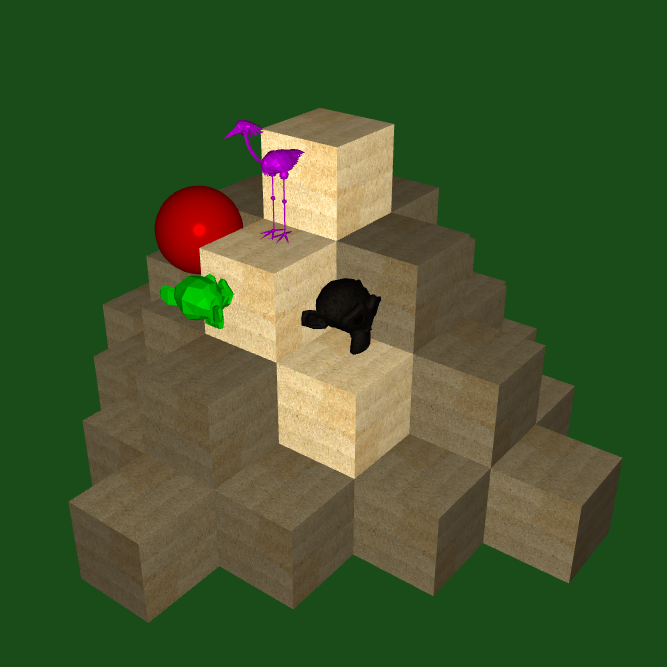
\includegraphics[width=14cm]{tebert.png}
  \caption{Tebert}
  \label{fig:tb}
\end{figure}


\end{document}